\section{S4.2: executed design, provenance and principal findings}
\label{sec:s42}
\textbf{Status: measured and independently reproduced.} Run \file{stage4\_s42\_all\_v1}, Slurm 924204 on s-004, completed the group, receiver-blocking, conditional-RI, backup, extension and mean-sensitivity workflow. The pinned model is unchanged. The runtime used PyTorch 2.14.0+cu126 and Transformers 4.51.3, with three independent two-GPU workers. All 51,904 records passed identity, checksum and exact-coverage checks; 44,754 were new endpoint measurements and 7,150 reused verified measurements. These are records, not a count of all forward passes: capture, mean construction and gates cost additional forwards.

The local audit reproduced all 49 exported numerical summary files, the adaptive decisions and the mean bank. All 16 root/measurement-worker gate reports passed their six-pair checks. It also checked cross-phase reuse, historical references, the downstream attention null, and that L26H31 diagnostics precede its own output replacement. The scientific population is still 89 discovery families, two orders each. The 20-family common panel selected subsequent measurements; the other 69 families provide additional discovery consistency, \emph{not untouched validation}. No held-out family or new model run was used for this report.

\begin{table}[htbp]\centering\small
\begin{tabular}{lrrr}\toprule
Phase & Records & New endpoints & Reused\\\midrule
Initial G1/blocking/K/G3 & 3,800 & 3,320 & 480\\
Conditional RI audit & 3,120 & 1,800 & 1,320\\
Triggered group refinements & 840 & 280 & 560\\
Selected discovery extensions & 22,072 & 17,282 & 4,790\\
Mean-replacement sensitivity & 22,072 & 22,072 & 0\\\midrule
Total & 51,904 & 44,754 & 7,150\\\bottomrule
\end{tabular}
\caption{Executed S4.2 measurement accounting. The G1/refinement/blocking registry used 71 distinct common configurations under its 128-configuration cap. Additional RI/background configurations have their own declared scope.}
\label{tab:s42_execution}
\end{table}

\subsection{What is established, and what remains an inference}
The data establish substantial joint head-group effects and live-model dependence of writer interventions on specified recipient groups. They also show that several conditional contributions survive a change of replacement baseline. They do \emph{not} yet establish a sufficient retained circuit, an individually validated membership list, or a complete composed chain.

The strongest organizing observations are:
\begin{enumerate}
\item L18H18 and L18H19 remain important inside several different groups. Their pair alone has a large joint effect; several larger groups are overlapping views of this same pair, not independent discoveries of separate circuits.
\item Clamping the seven O3 receivers removes about 88--90\% of the \emph{intervention effect} of L17H1's tested source masks. Clamping the L16H1/L16H21 pair similarly removes most of the L15H25 effect on the core panel. These are communication tests in a live model, not additive mediation shares.
\item The 23 residual RI heads collectively matter more in absolute family effect than the four fixed comparison cohorts, but their signed group effect changes with the replacement baseline. A collective RI effect does not assign the same role to every RI head.
\item L26H31 does not meet the backup retention rule in any of the five tested backgrounds. Upstream interventions change its attention, but this does not produce a substantial conditional answer effect.
\item The intervention baseline and fact order materially change the strength of group effects. Both must remain explicit in the later mechanism tests.
\end{enumerate}

\subsection{Metrics and limits of the sensitivity comparison}
Use the fixed clean-minus-corrupted first-divergent-token margin $M$. Noising has $I=M_c-M_{c,\mathrm{patched}}$; reverse restoration has $J=M_{r,\mathrm{patched}}-M_r$. A negative value remains a measured opposing contribution under that intervention. Orders are averaged within family, then families receive equal weight. Retention remains the frozen $0.10$-logit rule, including the heterogeneous-effect branch; it is not a significance test. Intervals are 20,000-draw whole-family bootstrap intervals, seed 20260923, and are descriptive after adaptive selection.

For a group $S$, $N(S)=I(S)-\sum_h I(h)$ measures nonadditivity and $\delta_h=I(S)-I(S\setminus\{h\})$ measures the additional effect of replacing $h$ when its partners are already replaced. A head left unpatched remains live and can change in response to upstream interventions. Neither $N$ nor $\delta$ alone proves redundancy, synergy in an information-theoretic sense, or sufficient backup.

Mean sensitivity uses the same declared configurations, with means indexed by head, textual fact slot, token role and within-name bucket. Means balance events within each family and then families, exclude the evaluated family, and fall back to less specific keys only with the prescribed family support. Demonstrations and the teacher-forced answer prefix stay live. For G2, donor Scope P covers the original prompt; the mean implementation replaces only eligible test positions. In particular, the ``restore'' direction with a mean is a \emph{corrupted-recipient sensitivity intervention}; it is not restoration from a clean donor. We therefore use it to assess baseline dependence, not as a second literal rescue experiment.

Some reused historical Scope-P records contain the exact margin effect but not both individual patched logits. They support the relevant margin and candidate-preference comparisons, but cannot retrospectively support a clean-logit versus distractor-logit decomposition. New endpoints contain both logits. Candidate accuracy here is a two-candidate first-divergent-token measure, not full-name generation accuracy.
\FloatBarrier

\section{G1: joint dependence, conditional roles and receiver blocking}
\label{sec:s42_g1}
\subsection{Eight groups, with shared measurements rather than eight independent circuits}
\begin{table}[htbp]\centering\footnotesize
\begin{tabular}{lp{.23\linewidth}p{.49\linewidth}r}
\toprule
ID & Pattern & Members & Configs \\
\midrule
O1 & L13H10 / sentence & L16H1, L17H3, L18H18, L18H19 & 9 \\
O2 & L15H25 / child-last & L16H1, L16H21 & 3 \\
O3 & L17H1 / mother & L18H18, L18H19, L18H24, L19H16, L20H1, L22H5, L27H6 & 15 \\
O4 & L17H3 / colon & L18H18, L18H19 & 3 \\
I1 & L27H6 / Q & L18H18, L18H19, L19H16, L20H1, L23H15, L25H17 & 13 \\
I2 & L21H23 / KV & L17H24, L18H18, L18H19, L19H16, L20H1 & 11 \\
I3 & L30H18 / Q & L18H18, L18H19, L20H1, L23H15, L25H17 & 11 \\
I4 & L18H18 / Q & L16H1, L16H21, L17H3 & 7 \\
\bottomrule
\end{tabular}

\caption{The eight executed G1 rosters. Every group member is replaced at the colon. The source masks in outgoing-group labels describe the route evidence motivating selection; they do not change the members' intervention site. I2 retains the provisional L17H24 nomination.}
\label{tab:s42_groups}
\end{table}

Singles, whole groups and group-minus-one interventions deduplicate to 49 base masks. The actual initial phase reused 480 historical F records: the L27H6 singleton was recomputed where G3 additionally required live attention diagnostics. Refinements reused many masks again. This is not an exhaustive subset search.

The extension cap selected 14 G1 contrasts and two L17H1 blocking contrasts, together with their matching constituent measurements. O2, I4 and most sign-split contrasts were retained on the core panel but not selected for extension; their absence from the extended schedule is a budget decision, not a null result. Several important summaries can nevertheless be recovered without another forward pass: a saved whole-group effect on all 89 families and the compatible historical F singles are enough to compute donor-noising $N(S)$ for six groups. These additional CPU contrasts are marked explicitly in Table~\ref{tab:s42_group_effects}. They do not create missing reverse or mean-single measurements.

\begin{table}[htbp]\centering\small
\begin{tabular}{lrrrrl}
\toprule
Group & $n_f$ & $I(S)$ & $N(S)$ & $\E|N_f|$ & Interaction label \\
\midrule
O1 & 89 & +5.737 & -0.519 & 0.738 & coherent \\
O2 & 20 & +1.842 & +0.104 & 0.122 & coherent \\
O3 & 89 & +6.528 & -0.391 & 1.228 & heterogeneous \\
O4 & 89 & +5.630 & -0.173 & 0.564 & heterogeneous \\
I1 & 89 & +5.340 & +1.575 & 1.627 & coherent \\
I2 & 89 & +5.461 & +1.585 & 1.595 & coherent \\
I3 & 89 & +5.574 & +0.981 & 1.119 & coherent \\
I4 & 20 & +1.718 & +0.387 & 0.387 & coherent \\
\bottomrule
\end{tabular}

\caption{Group noising effects and nonadditivity. The six 89-family interaction rows are additional CPU derivations from measured whole groups and compatible saved F singles. O2 and I4 remain 20-family results. All effects are in logits. ``Heterogeneous'' is the frozen retention label, even when a descriptive signed-mean interval excludes zero.}
\label{tab:s42_group_effects}
\end{table}

O4, the pair \{L18H18,L18H19\}, has mean $I=5.630$ on 89 families. Adding L16H1 and L17H3 in O1 gives $5.737$; this small difference is not evidence that those two heads are universally dispensable. O1 contains additional, already-intervened downstream heads, and its conditional L16H1 effect is much smaller than that head's effect inside the upstream pair O2. O3 reaches $6.528$ but mixes positive and opposing contributors. The I1--I3 group effects, $5.340$, $5.461$ and $5.574$, are also dominated by shared layer-18 structure. Their overlap prevents treating their effects as separate pieces that can be added into a circuit score.

The new 89-family CPU interaction means are $-0.519$ for O1, $-0.391$ for O3, $-0.173$ for O4, and $+1.575,+1.585,+0.981$ for I1--I3. For example, I1 has a descriptive interval $[1.335,1.827]$. O4 has signed interaction $-0.173$ but mean absolute family interaction $0.564$: average near-additivity would hide nontrivial variation. These are useful constraints on a joint mechanism, not proof that each recipient consumes an independent message.

\subsection{Conditional roles change with the surrounding group}
\begin{figure}[htbp]\centering
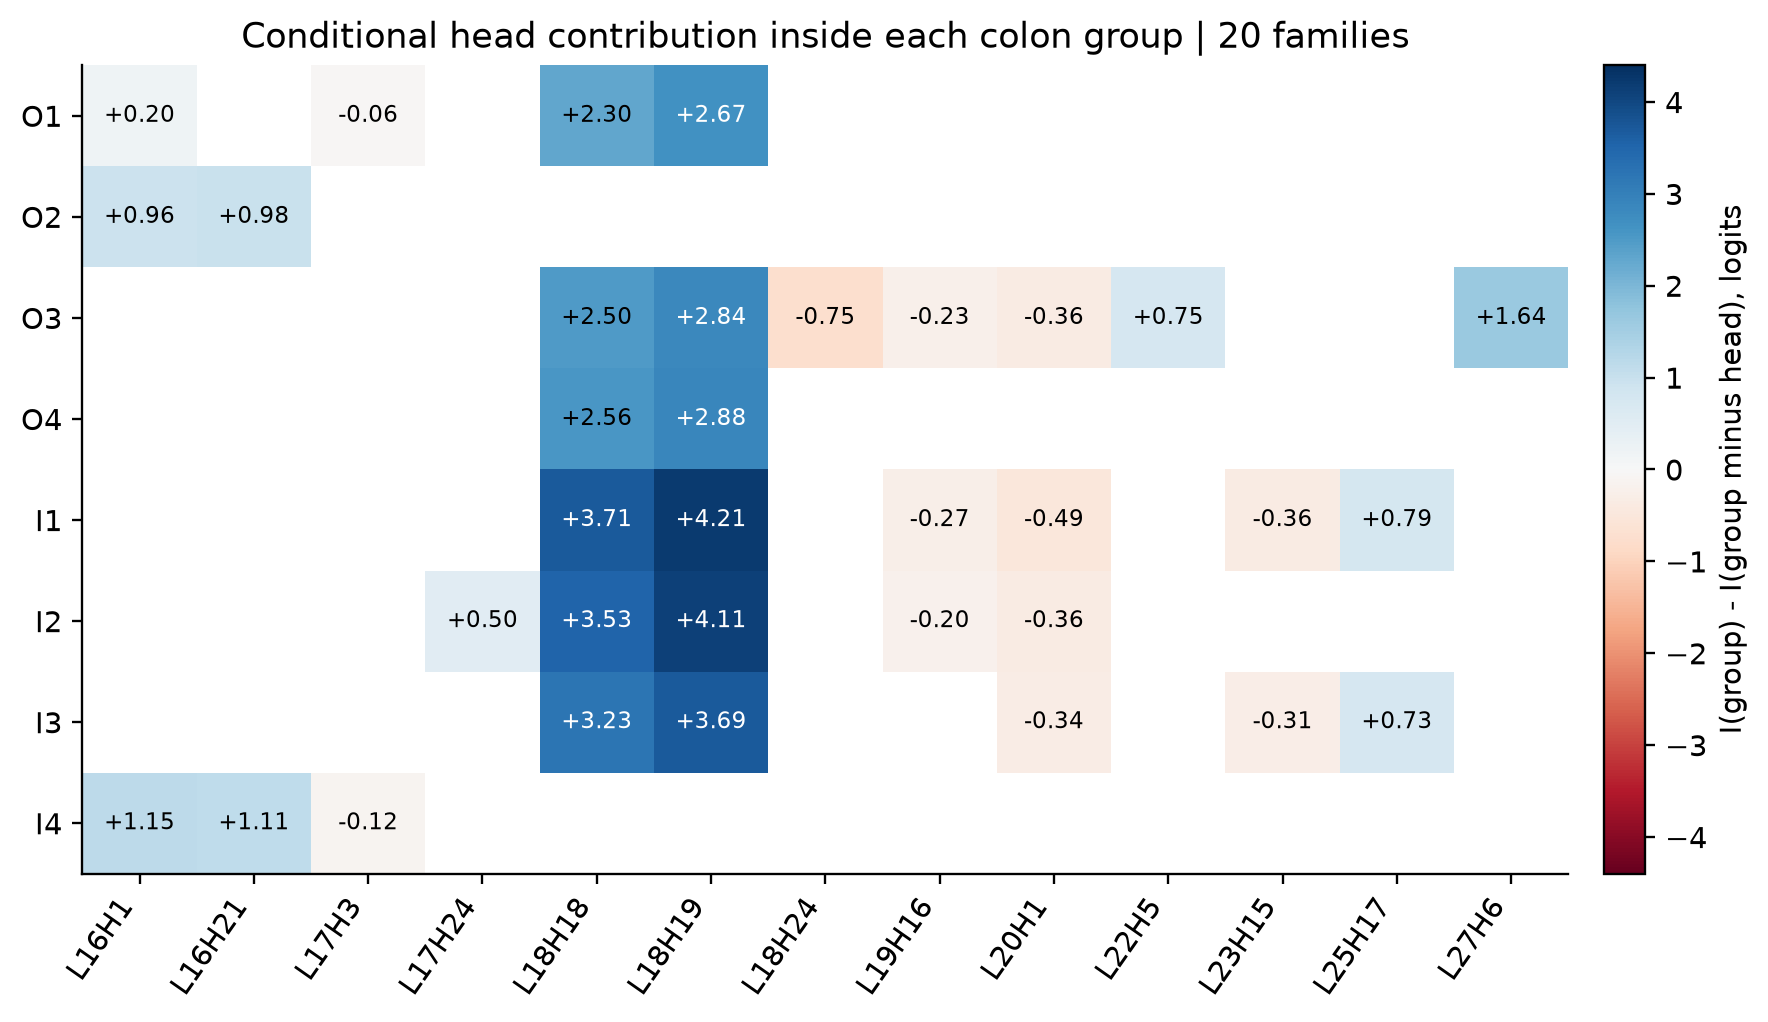
\includegraphics[width=\linewidth]{figures/s42_conditional_heatmap.png}
\caption{Core-panel conditional contributions. Blank entries are nonmembers, not measured zeros. The same head has a different background in each row, so changes across rows are evidence of context dependence. Rows overlap substantially.}
\label{fig:s42_conditional}
\end{figure}

Within I1, conditional effects of L18H18 and L18H19 are $3.706$ and $4.214$ on the core panel; within O4 they are $2.559$ and $2.875$. Inside I1, the opposing L19H16, L20H1 and L23H15 effects remain negative, while L25H17 contributes positively. Removing such negative contributions may improve a margin, but excluding them from an explanation can reduce fidelity to the full model.

The child-reader pair O2 has joint effect $1.842$ and conditional contributions $0.961$ and $0.985$. I4 adds L17H3; its effect is $1.718$, with a negative conditional L17H3 contribution. By contrast, inside O1 the conditional L16H1 effect is only $0.197$, and L17H3 is below the rule at $-0.065$. A plausible explanation is that downstream replacement can mask an upstream contribution; these measurements do not distinguish all serial and parallel alternatives.

The sign-partition interaction $I(S)-I(S_+)-I(S_-)$ is $2.285$ for I1, $1.754$ for I2, $1.831$ for I3 and $1.658$ for O3 on the core panel. These partitions follow the measured singleton signs; they are not independent biological categories. Their substantial interactions motivate keeping opposing groups in the later completeness audit. The large L18H18/L18H19 conditional effects retained in the extension remain positive under both mean directions. This supports their prioritization; it still does not establish that the pair is a sufficient retained mechanism.

\subsection{Order and baseline sensitivity change the interpretation of necessity}
\begin{figure}[htbp]\centering
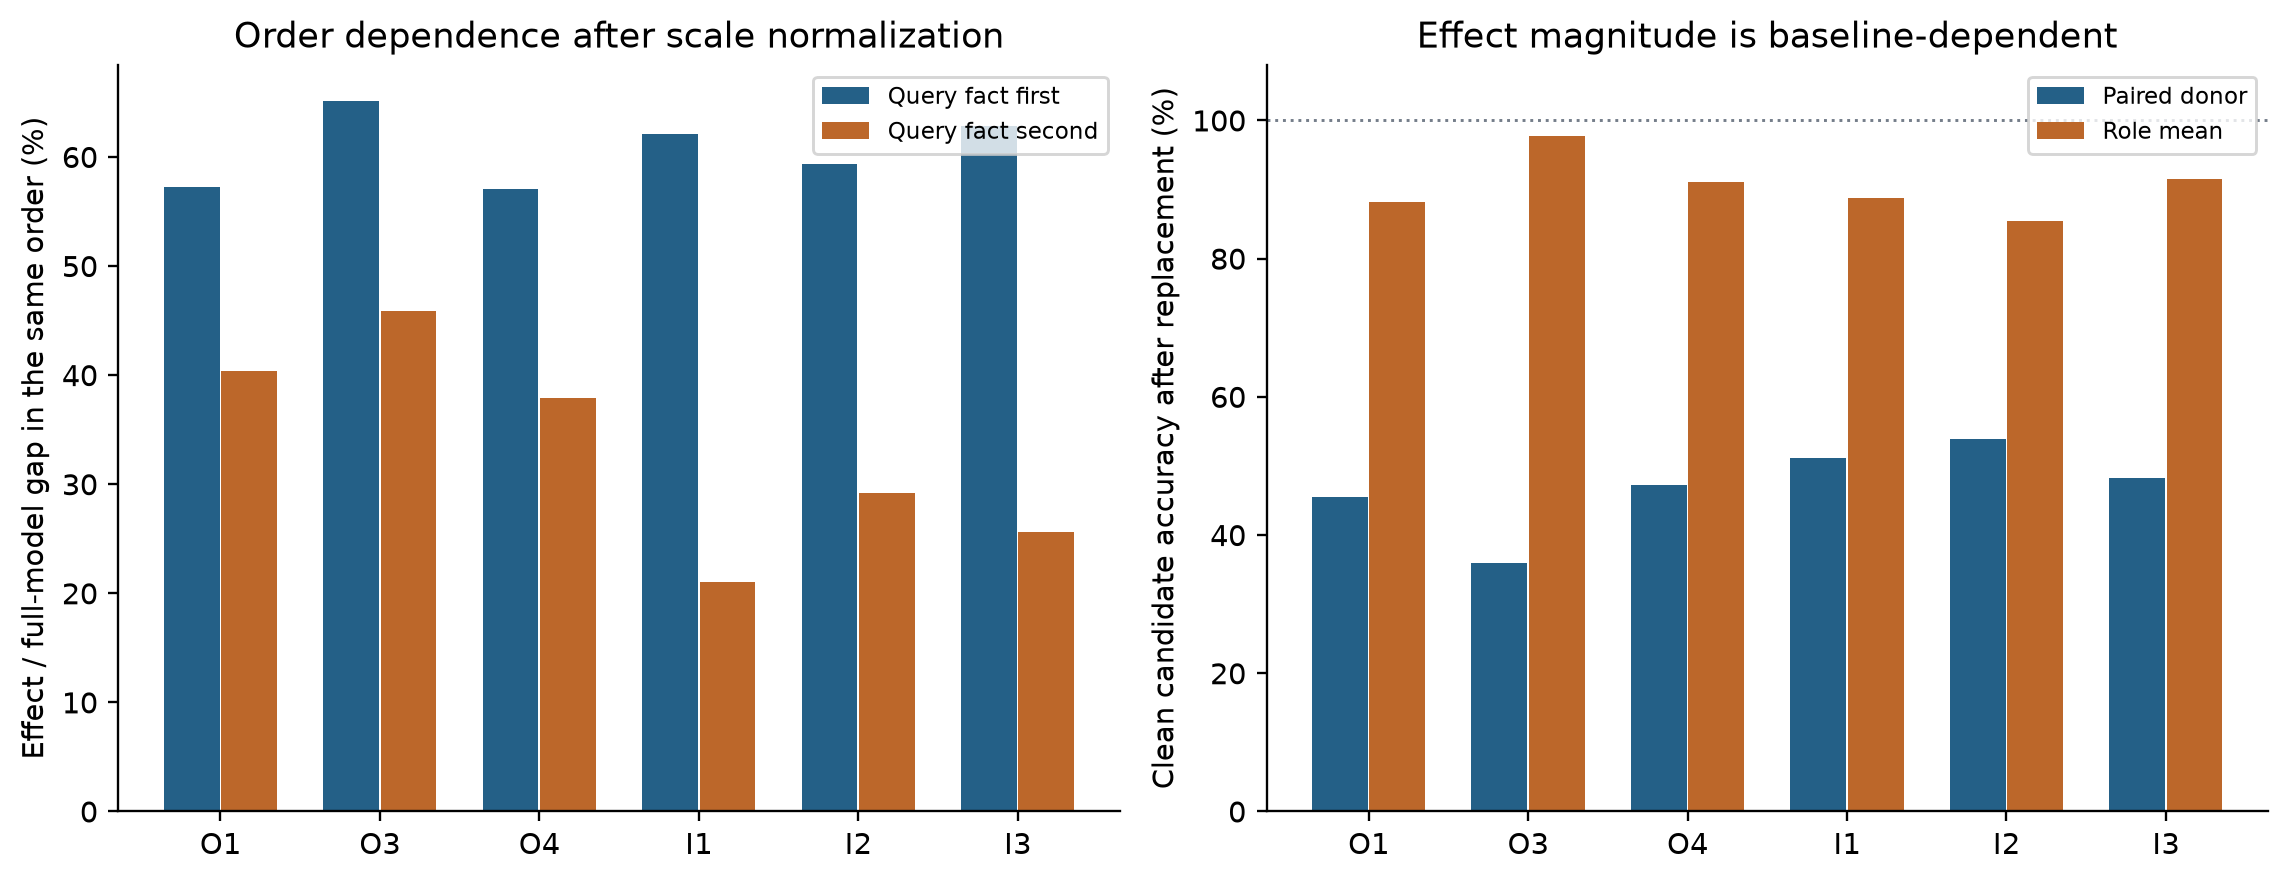
\includegraphics[width=\linewidth]{figures/s42_order_accuracy.png}
\caption{Six extended groups on 89 families. Left: effects are divided by the full-model clean-minus-corrupted gap for the \emph{same order}. Right: clean candidate accuracy after group replacement. The intact accuracy is 100\%. The two replacement baselines are different interventions, not two estimates of one uniquely defined necessity score.}
\label{fig:s42_order_accuracy}
\end{figure}

The full-model gap is itself order-dependent: $14.575$ when the queried fact comes first and $7.765$ when it comes second. Raw group effects must be interpreted against this difference. O3 falls from $9.497$ to $3.560$ logits, equivalent to $65.2\%$ versus $45.8\%$ of the respective gaps. I1 falls from $9.046$ to $1.633$, or $62.1\%$ versus $21.0\%$. Normalization reduces the apparent disparity, but does not remove it. The same phenomenon is present under role means. Order robustness is therefore an informative group-level question for S4.4, not an already settled property.

Under paired-donor noising, O3 replacement leaves only $36.0\%$ clean candidate accuracy; under role means it leaves $97.8\%$. For O4 these values are $47.2\%$ and $91.0\%$. The groups still have substantial mean-baseline margin effects, but the claim ``removing this group destroys the task'' would depend strongly on how removal is defined. A corrupted donor can transmit the competing binding, while a mean need not do so. The present evidence supports that interpretation as a hypothesis, not a demonstrated decomposition of the difference.

This disparity is not simply a smaller unprojected perturbation for O3: the mean joint head-output change norm is $6.580$ with donors and $6.686$ with means. These norms are descriptive and do not control downstream nonlinear amplification or direction. For RI23, in contrast, the norms differ substantially ($13.984$ versus $29.955$); its sensitivity comparison is also not norm matched. We will preserve both baselines and the performance guards in S4.5.

\subsection{Receiver blocking confirms dependence on specified recipients}
\begin{figure}[htbp]\centering
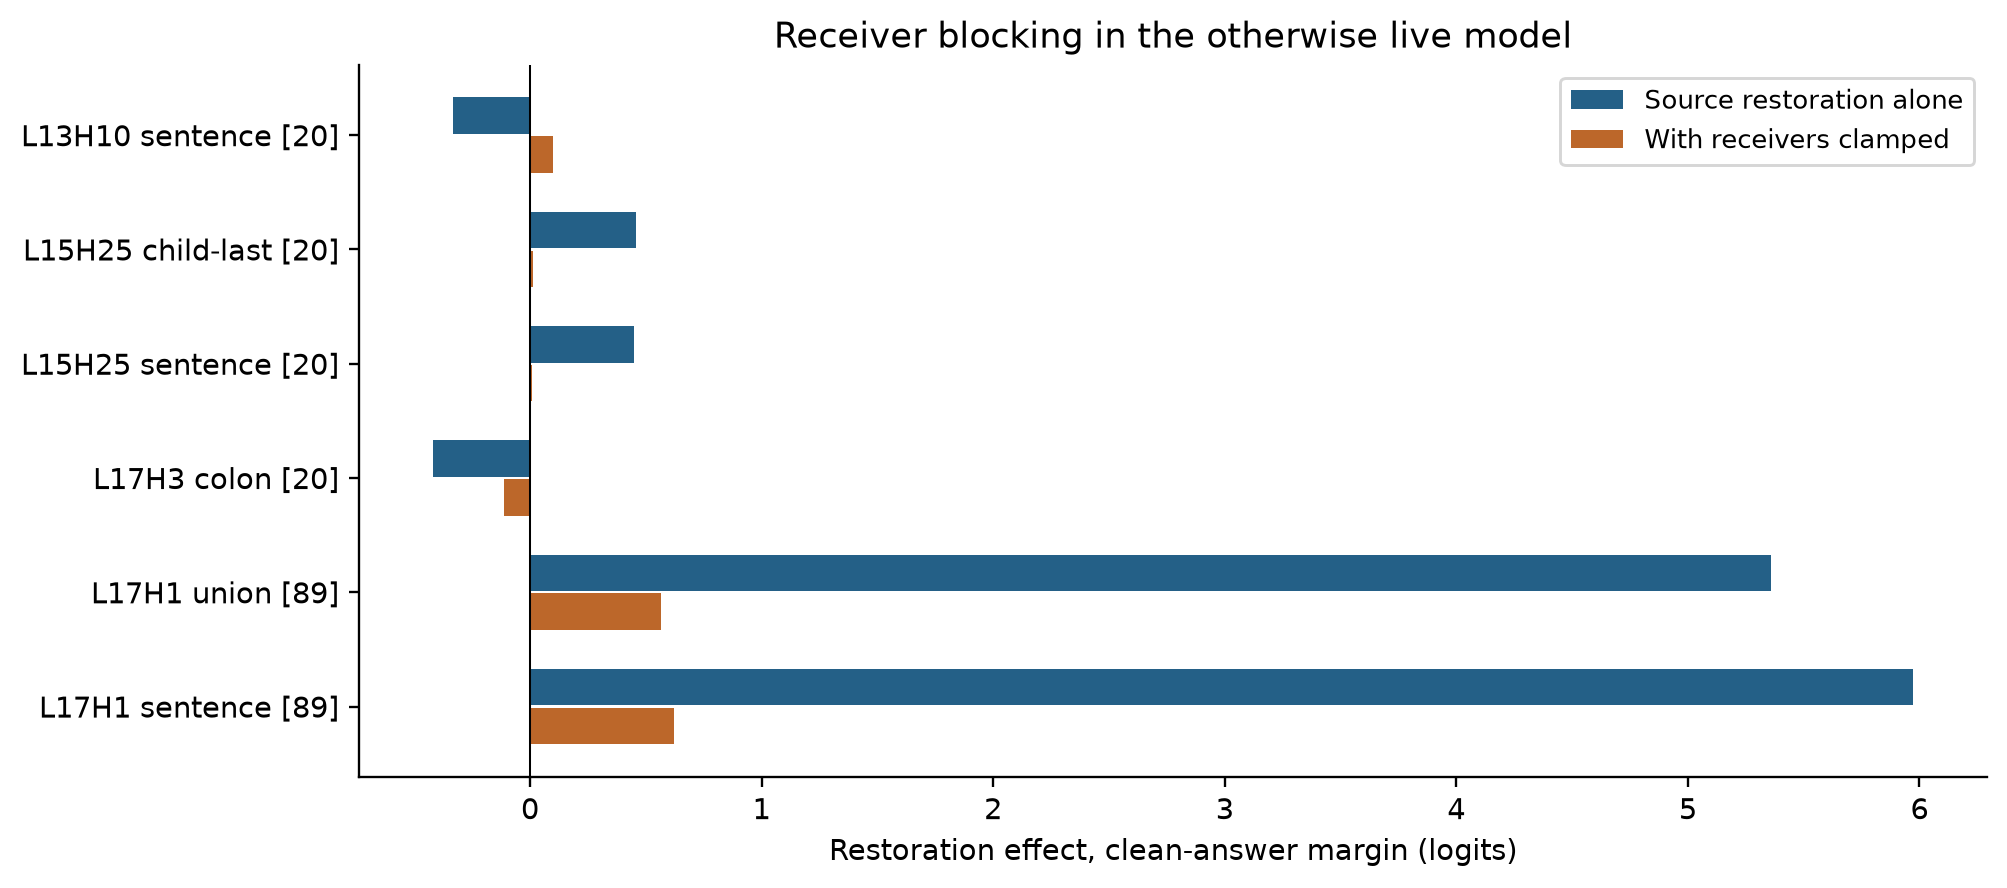
\includegraphics[width=\linewidth]{figures/s42_blocking.png}
\caption{Source restoration before and after clamping the specified recipients' colon outputs to their original corrupted values. The difference is $B$. Bracketed sample sizes distinguish the core-only and extended patterns. Negative source effects remain negative evidence; a ratio exceeding one is possible and does not describe a probability or mediated share.}
\label{fig:s42_blocking}
\end{figure}

\begin{table}[htbp]\centering\small
\begin{tabular}{llrrrr}
\toprule
Source & Mask & $n_f$ & $J_W$ & $B$ & $B/J_W$ \\
\midrule
L13H10 & sentence & 20 & -0.330 & -0.429 & 129.9\% \\
L15H25 & child-last & 20 & +0.457 & +0.442 & 96.7\% \\
L15H25 & sentence & 20 & +0.451 & +0.442 & 97.8\% \\
L17H3 & colon & 20 & -0.417 & -0.304 & 72.9\% \\
L17H1 & writer-union & 89 & +5.358 & +4.790 & 89.4\% \\
L17H1 & sentence & 89 & +5.972 & +5.351 & 89.6\% \\
\bottomrule
\end{tabular}

\caption{Paired-donor restoration and receiver blocking. Ratios are ratios of matched means. The companion data file provides jointly bootstrapped ratio intervals and the opposite intervention direction.}
\label{tab:s42_blocking}
\end{table}

On all 89 families, restoring L17H1's writer union gives $J_W=5.358$; O3 clamping removes $B=4.790$, leaving $0.568$. The ratio is $89.4\%$. For the whole query sentence, $J_W=5.972$, $B=5.351$ and the residual is $0.621$, a ratio of $89.6\%$. Noising gives closely corresponding ratios of $87.9\%$ and $88.2\%$. These measurements establish that the specified recipient outputs must be allowed to respond for most of this source intervention effect in the tested background. The remaining effect can reflect unblocked paths, interactions or other live computations; it is not a measured exclusive alternative route.

The L15H25 child-last and sentence tests give restoration blocking ratios of $96.7\%$ and $97.8\%$ on the core panel. This is strong motivation for the explicit ordered L15H25--\{L16H1,L16H21\}--\{L18H18,L18H19\} test, but it is not that test itself. The single-head path results and the group blocking result cannot be multiplied into a chain effect.

L13H10 and L17H3 have negative source and blocking effects. For L13H10 the blocking ratio exceeds one; clamping can remove an opposing influence and reveal a small residual of the opposite sign. This directly illustrates why $B/J_W$ is an intervention ratio and cannot be interpreted as a unique fraction of information flow. All self-clamp controls remain zero. L17H1 blocking retains under mean replacement as well, with smaller effects; this supports a baseline-robust dependency while preserving the distinction between mean sensitivity and donor rescue.
\FloatBarrier

\section{G2: conditional RI participation without a uniform RI mechanism}
\label{sec:s42_g2}
\subsection{The chosen weakened background is mild enough to interpret}
The measured prefix rule selected $K=\{\mathrm{L21H18}\}$. It leaves $66.4\%$ of the symmetric clean-minus-corrupted gap, using $(G-I_K-J_K)/G$ on the common panel. The two- and three-head prefixes leave $45.3\%$ and $31.6\%$, but the rule selects the smallest qualifying prefix. The full four-head prefix reverses the gap ($-11.4\%$); it would be a poor default for identifying modest backups. No floor warning was needed for the selected K.

For each RI head, the candidate uses its original-prompt mask, while K uses the colon. Comparing this conditional effect to the saved intact Scope-P effect is valid; substituting colon-only singles would not be. All 31 candidates were measured on the common panel. Fourteen were extended, including the eight previously strong RI heads and six additional retained candidates. None of the seventeen unextended candidates is thereby proved irrelevant in every context.

\begin{figure}[htbp]\centering
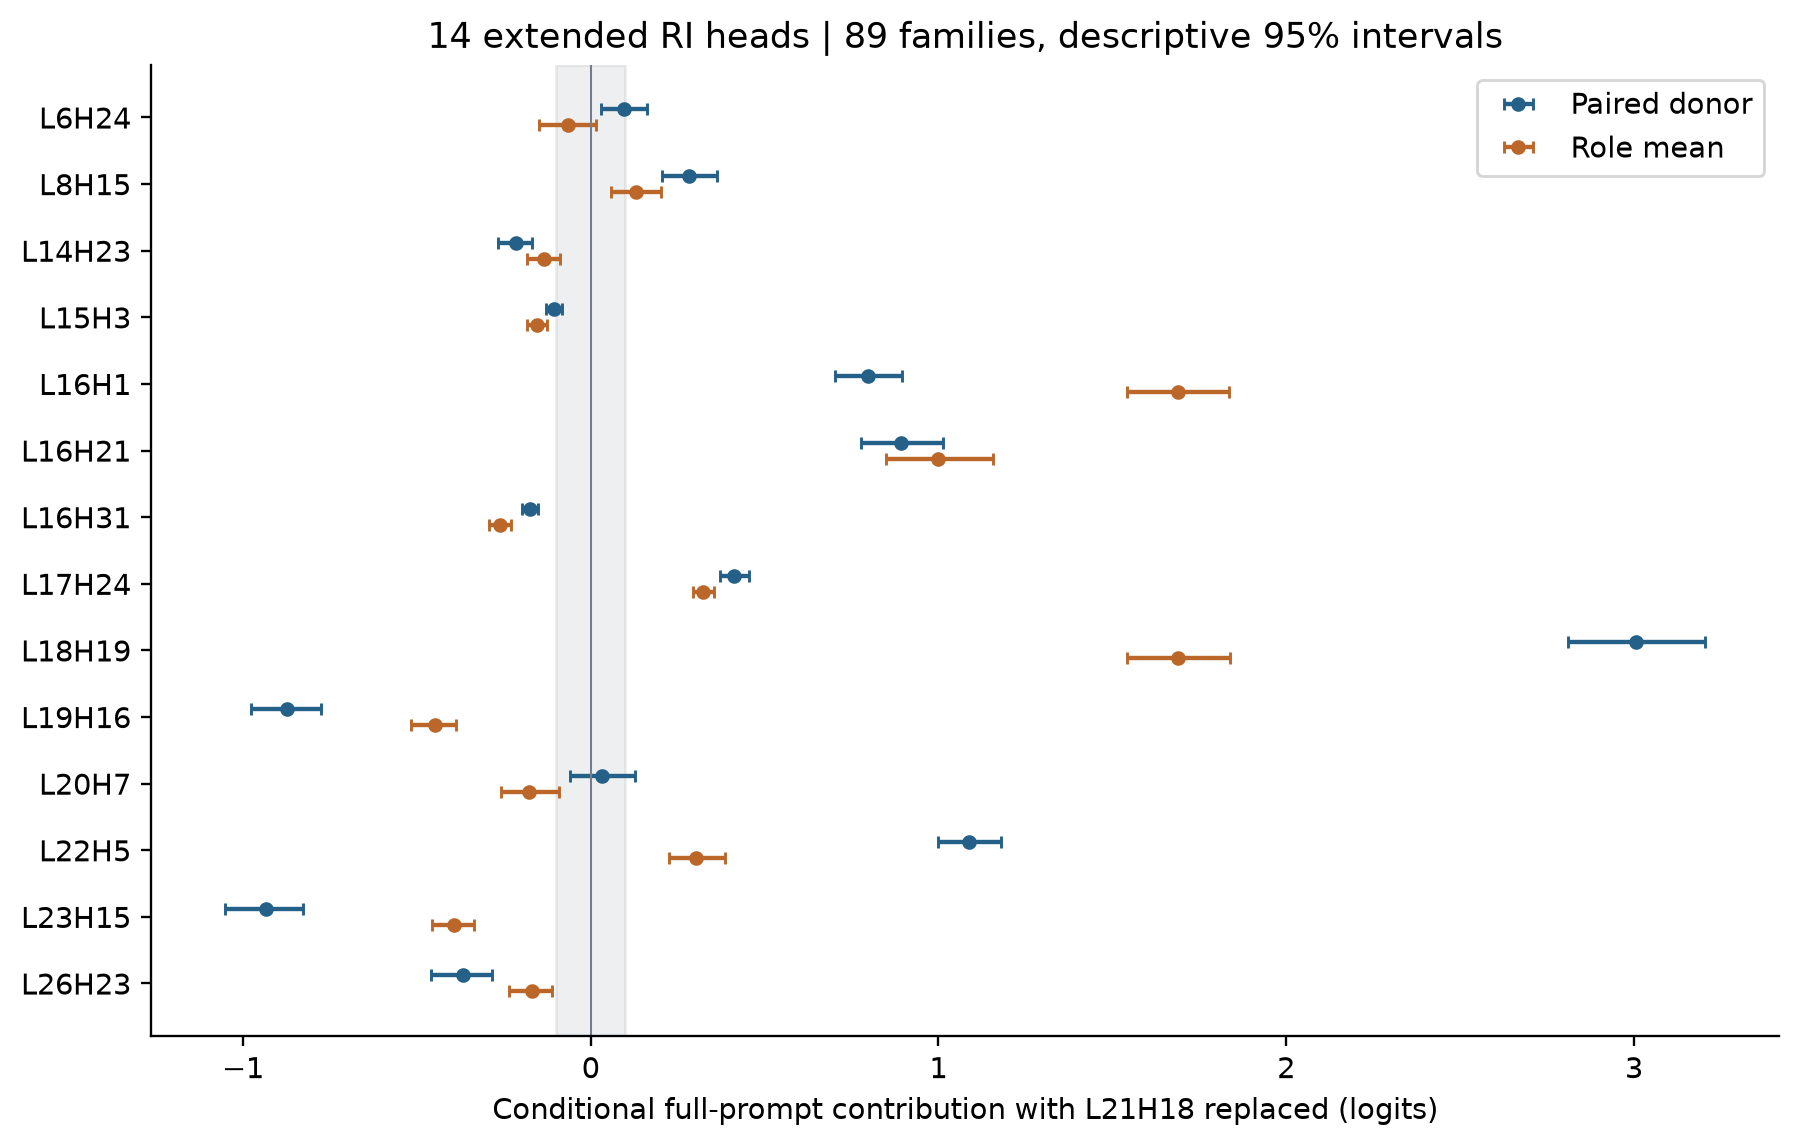
\includegraphics[width=\linewidth]{figures/s42_ri_heads.png}
\caption{Extended conditional contributions under paired donors and means. The shaded band marks the practical $\pm0.10$ threshold, not a confidence region. Signed means alone do not capture heterogeneous heads such as L6H24 and L20H7.}
\label{fig:s42_ri}
\end{figure}

\begin{table}[htbp]\centering\small
\begin{tabular}{lrrrrr}
\toprule
Head & $I_{K}$ & $J_{K}$ & $I_{K,\mu}$ & $\E|I_{K,f}|$ & $I_K-I_0$ \\
\midrule
L6H24 & +0.096 & +0.103 & -0.065 & 0.241 & -0.005 \\
L8H15 & +0.284 & +0.316 & +0.130 & 0.379 & +0.005 \\
L14H23 & -0.215 & -0.201 & -0.134 & 0.246 & -0.003 \\
L15H3 & -0.104 & -0.086 & -0.154 & 0.115 & +0.002 \\
L16H1 & +0.798 & +0.769 & +1.688 & 0.803 & -0.070 \\
L16H21 & +0.893 & +0.999 & +0.999 & 0.899 & -0.032 \\
L16H31 & -0.173 & -0.167 & -0.261 & 0.174 & +0.014 \\
L17H24 & +0.413 & +0.413 & +0.324 & 0.413 & -0.020 \\
L18H19 & +3.006 & +3.129 & +1.689 & 3.006 & -0.066 \\
L19H16 & -0.874 & -0.893 & -0.448 & 0.874 & -0.054 \\
L20H7 & +0.032 & +0.099 & -0.177 & 0.318 & +0.058 \\
L22H5 & +1.088 & +1.115 & +0.304 & 1.088 & +0.105 \\
L23H15 & -0.933 & -0.902 & -0.394 & 0.933 & +0.014 \\
L26H23 & -0.367 & -0.354 & -0.167 & 0.376 & +0.001 \\
\bottomrule
\end{tabular}

\caption{Fourteen extended RI candidates on 89 families. $I_K$ and $J_K$ use paired donors; $I_{K,\mu}$ is mean sensitivity in clean recipients. The final column is the paired donor change from the intact Scope-P effect. The full ledger includes labels, intervals and the corrupted-recipient mean direction.}
\label{tab:s42_ri}
\end{table}

\subsection{Conditional importance is usually not a newly unmasked backup}
The five positive strong RI heads remain positive and the three negative strong heads remain opposing under both replacement baselines. Their precise effects change, but their directions are stable. In the selected K background, L18H19 remains the largest positive RI single at $3.006$; L22H5 gives $1.088$; L19H16, L23H15 and L26H23 give $-0.874,-0.933,-0.367$.

Most changes from the intact-model effect are small. The donor change for L22H5 is $+0.105$, just above the practical signed threshold, while L18H19 has signed change $-0.066$ but mean absolute change $0.250$. Mean replacement reduces or removes several of these changes. Thus the audit mostly confirms participation in a weakened background; it does not reveal a broad population of previously silent backups. A retained conditional effect and a retained \emph{increase} in that effect answer different questions.

The six additional candidates form the explicit follow-up set
\[
R_6=\{\mathrm{L6H24,L8H15,L14H23,L15H3,L16H31,L20H7}\}.
\]
Their status is not uniform:
\begin{itemize}
\item L8H15 has positive donor conditional means in both directions ($0.284,0.316$), but mean replacement yields heterogeneous rather than coherent effects. Its earlier Scope F was essentially zero while Scope P was positive: a colon-only route search would miss its relevant positional scope.
\item L14H23 is opposing under donors and heterogeneous under means. L16H31 remains opposing across the tested directions/baselines and has prior P and F of similar magnitude, supporting a focused colon-source follow-up.
\item L15H3 is borderline: donor noising retains at $-0.104$, but donor restoration is $-0.086$ with mean absolute effect $0.097$, below the rule. Its inclusion in the starting head set is conservative and provisional.
\item L6H24 and L20H7 have cancellation across families. L20H7 changes from donor mean $+0.032$ to mean-baseline $-0.177$, while remaining substantial in absolute family effect. Neither should receive a fixed positive-reader label from the donor mean.
\end{itemize}

These heads are conditional-contribution candidates, not yet individually route-supported semantic members. For cost control, the local expansion prioritizes L8H15 and the colon-localized L16H31/L20H7; L6H24, L14H23 and L15H3 remain in grouped mechanism tests without a broad search for their routes. L26H23 receives a late local-route check because its robust opposing contribution is still insufficiently connected to the existing map.

\subsection{RI23 has a collective signal, with cancellation and baseline sensitivity}
The residual set is the original RI31 minus the eight strong RI heads, not the 23 rank-selected heads. In the intact background, its 89-family donor group effect is $+0.116$, but its mean absolute family effect is $0.594$. Under K these become $+0.185$ and $0.656$. The four layer-matched reference groups have mean absolute effects averaging $0.215$ and $0.197$, respectively. The paired difference in family magnitudes is $0.379$ with descriptive interval $[0.280,0.488]$ in the intact background, and $0.459$ with $[0.353,0.579]$ under K.

\begin{figure}[htbp]\centering
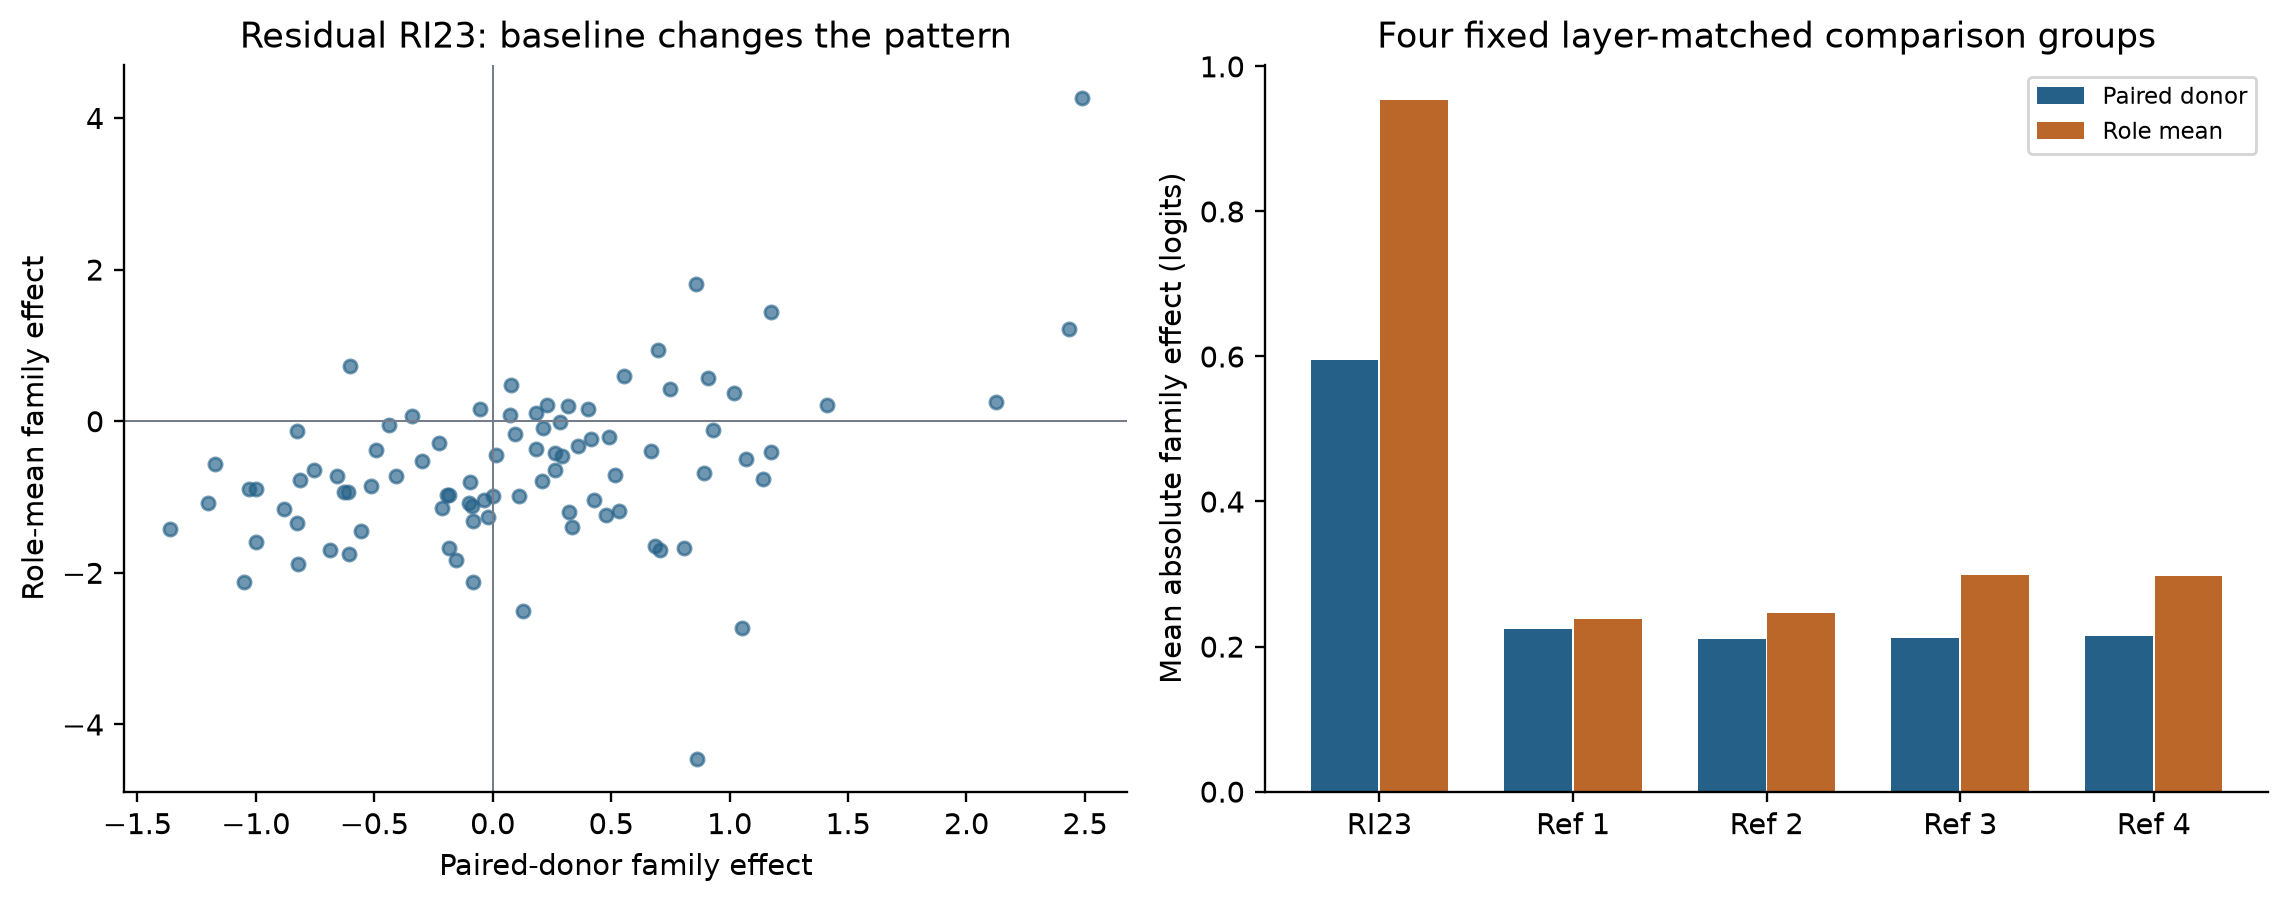
\includegraphics[width=\linewidth]{figures/s42_residual.png}
\caption{Residual RI23 versus the four fixed reference cohorts. Left: each point is one family's intact-background group effect under the two replacement baselines. Right: absolute effects retain information hidden by signed cancellation. These four cohorts are descriptive comparisons, not a sampled null distribution or a calibrated RI-specificity test.}
\label{fig:s42_residual}
\end{figure}

Under means, the intact RI23 signed effect becomes $-0.633$, with mean absolute effect $0.954$; under K it is $-0.636$ and $0.979$. The group is still more disruptive in absolute effect than the comparison cohorts, but the donor story of a weak positive average does not survive as a baseline-independent directional claim. Its donor intact nonadditivity, computed using saved Scope-P singles, is $+0.186$ with interval $[0.129,0.249]$. Therefore summing individual RI effects would not recover the group result either.

The reference groups themselves are not null: all four meet the heterogeneous retention rule in the extended donor panel. Layer matching controls a particular compositional difference; it does not match norms or every behavioral property. RI23 also has a larger output perturbation norm, especially under means. Consequently, the results support a \emph{collectively relevant, heterogeneous RI remainder}, not a claim that RI alone uniquely identifies the relational mechanism. The group-only fact-by-query panel will test whether this collective signal follows the task's binding/query structure.
\FloatBarrier

\section{G3: the L26H31 backup hypothesis is not supported in the tested panel}
\label{sec:s42_g3}
The five backgrounds are intact, K1=\{L21H18\}, K3=\{L21H18,L22H5,L21H6\}, K4=K3$\cup$\{L27H6\}, and L27H6 alone. The conditional colon effects are $0.0049,0.0071,0.0078,0.0239,0.0206$ logits. Their mean absolute family effects range from $0.026$ to $0.040$, all below $0.10$. No G3 contrast triggered extension, reverse restoration or mean sensitivity. The different Scope-P G2 test also failed to retain L26H31 on the core panel.

\begin{figure}[htbp]\centering
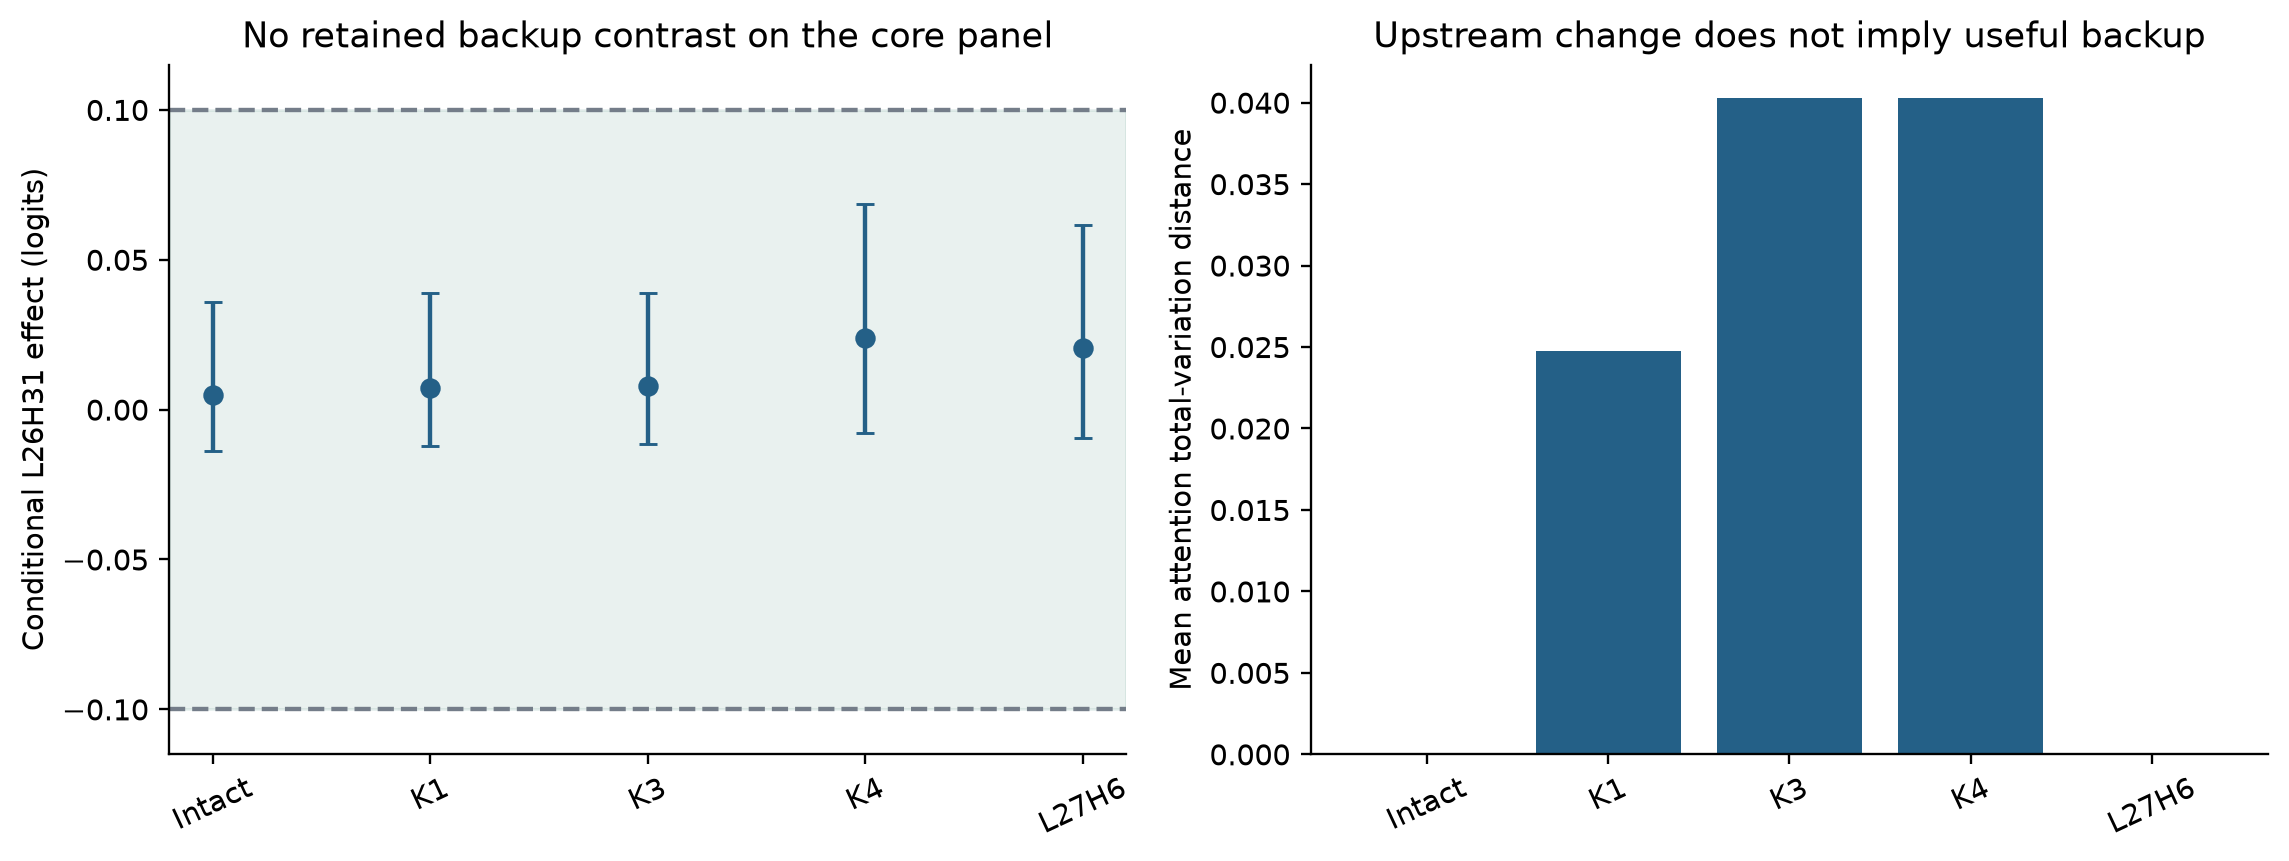
\includegraphics[width=\linewidth]{figures/s42_g3.png}
\caption{The backup test used 20 discovery families and two orders. Attention distances are measured before L26H31's own replacement. K3 and K4 produce identical earlier-head diagnostics; downstream L27H6 alone produces exactly zero attention/output change, as required by layer causality. These null checks do not force the downstream answer contrast to be zero.}
\label{fig:s42_g3}
\end{figure}

Removing K3 changes attention by mean total-variation distance $0.0403$ and the head output by mean relative norm $0.0960$. Adding the downstream L27H6 intervention changes the conditional answer effect, but cannot change this already computed attention/output. Thus attention reorganization is observable without a useful backup effect by the frozen rule.

\textbf{Decision:} retire L26H31 as a dedicated backup target in the next mandatory panel. This is a bounded negative result on the tested backgrounds and sample, not a universal absence claim. It can remain inside the predeclared residual RI group. If the limited whole-group addback described below is triggered, it enters only as one member of that group, not as a revived individually supported backup.
\FloatBarrier

\section{Integrated interpretation: observations, hypotheses and limits}
\label{sec:s42_interpretation}
\textbf{Observation 1: a common layer-18 pair participates across several groups.}
The pair's joint intervention, conditional effects and recipient-blocking context support its centrality in the tested computation. \emph{Hypothesis:} the child-reader path and the L17H1 fact-writing path converge on this pair. \emph{Missing test:} the ordered multi-step interventions in S4.3. The current evidence does not establish that the separately measured arrows compose unchanged.

\textbf{Observation 2: opposite-sign contributors remain important inside groups.}
Positive incoming-group nonadditivity and sign-split interactions show that these heads are not explained by independent signed contributions. \emph{Hypothesis:} the mechanism balances competing bindings or readout directions in an order-dependent way. This is a functional possibility, not a measured representational interpretation. The group-only S4.4 panel and S4.5 completeness comparisons can separate a useful explanatory balance from merely score-improving deletions.

\textbf{Observation 3: large donor damage does not imply mean-ablation indispensability.}
O3 and O4 strongly affect margins with both baselines but preserve much higher accuracy under means. \emph{Hypothesis:} injecting the competing binding is more disruptive than replacing it with an averaged state. Similar O3 perturbation norms make a pure size explanation insufficient, but do not identify the relevant direction. This motivates symmetric baseline sensitivity and all-head-mean controls in S4.5 rather than declaring an already sufficient or necessary circuit.

\textbf{Observation 4: RI is neither uniformly causal nor uniformly irrelevant.}
Eight established RI heads remain signed contributors, six additional candidates need qualified treatment, the residual group has substantial family effects, and L26H31 fails the proposed backup criterion. Many important writers and readers are non-RI. The warranted conclusion is partial, heterogeneous overlap between RI selection and the causal mechanism. A held-out membership conclusion still requires frozen routes/backgrounds and the specified validation criteria.

\textbf{Observation 5: positional context matters beyond changes in full-model confidence.}
The normalized order contrast persists, especially for the incoming groups. \emph{Hypothesis:} the selected groups bear different amounts of the computation when the target fact is earlier versus later. The alternative that other live pathways compensate in one order remains viable. This is why later completeness tests compare the \emph{same group removal} in the full model and retained mechanism across both orders.

\textbf{Bounded claims.} No result here proves a complete semantic circuit, unique minimality, a universal relation detector, or an excluded head's irrelevance. Core-only and unextended results remain labelled as such. The new CPU-derived interactions are discovery analyses of already measured terms. The next plan is prospective and has no GPU results attached to it.

\section{Revised S4.3--S4.5: exact rosters, shared measurements and dependencies}
\label{sec:next_plan}
This section adopts the requested scope changes. It replaces the previous broad-search extension with \emph{one bounded local expansion}; S4.4 operates only on groups or retained mechanisms. S4.4 and S4.5 share one measurement registry and execution pipeline, while keeping distinct analytical questions. This supersedes the corresponding future-design choices in the earlier protocol; it does not retroactively alter the executed S4.1/S4.2 rules. The exact sets and conditional rules are also supplied in \file{data/s42_next_stage_plan.json}. No follow-up GPU implementation or submission was performed for this report.

\subsection{Fixed starting sets}
The initial retention candidate $C_0$ has 33 heads: the prior 25 strong heads, coverage candidates L13H18/L24H19, and the six conditional RI candidates $R_6$. Inclusion is deliberately conservative; it is not a declaration that all 33 are confirmed members. The following disjoint blocks completely enumerate $C_0$ and define the proposed group-first reduction units.

\begin{longtable}{p{.08\linewidth}>{\raggedright\arraybackslash}p{.64\linewidth}>{\raggedright\arraybackslash}p{.20\linewidth}}
\toprule Block & Exact heads & Rationale\\\midrule\endhead
$W$ & L15H25, L17H1 & Writers\\
$D$ & L16H1, L16H21 & Child readers\\
$P$ & L18H18, L18H19 & Shared pair\\
$A$ & L21H6, L21H18, L22H5, L27H6 & Late readers\\
$N$ & L13H10, L17H3, L18H24, L19H16, L20H1, L23H15, L26H23, L30H18 & Prior opposing set\\
$R_6$ & L6H24, L8H15, L14H23, L15H3, L16H31, L20H7 & Conditional audit\\
$T$ & L14H26, L17H17, L17H24, L19H22, L21H23, L25H17, L30H13 & Other strong heads\\
$U$ & L13H18, L24H19 & Coverage candidates\\\bottomrule
\end{longtable}
These are practical reduction units; in particular $T$ and $U$ are not asserted to be homogeneous functional modules. The eight negative-labelled heads in $N$ are selected by prior effects; their signs are not assumed invariant in a reduced mechanism.

The initial RI subset is
\begin{quote}\small
L6H24, L8H15, L14H23, L15H3, L16H1, L16H21, L16H31, L17H24, L18H19, L19H16, L20H7, L22H5, L23H15, L26H23.
\end{quote}
The other 19 heads in $C_0$ are
\begin{quote}\small
L13H10, L13H18, L14H26, L15H25, L17H1, L17H3, L17H17, L18H18, L18H24, L19H22, L20H1, L21H6, L21H18, L21H23, L24H19, L25H17, L27H6, L30H13, L30H18.
\end{quote}
For any later mask $C$, ``RI members'' means $C\cap R_{31}$ and ``non-RI members'' means $C\setminus R_{31}$, with the exact retained roles recorded. They are not silently held at 14 and 19 after reduction.

\subsection{S4.3: a single exact local expansion, with no broad candidate screen}
\textbf{Purpose.} Test the remaining most informative local routing questions and whether the two proposed chains actually compose. We omit the all-1,024-head/32-MLP attribution screen, its 48-candidate calibration, the inventory/block fallback scan and automatic EAP expansion. Stopping with an unresolved source is acceptable. It means that this bounded map is incomplete, not that the source was disproved.

\textbf{Exact intervention semantics.} As in S4.1, start from a source-replaced hybrid with other downstream residual increments frozen after their normalization. Release only the named MLPs/blocks or specified head outputs, recapture the receiver's actual Q/K/V, and inject the selected channel into a fresh recipient. Compare with the same source/site/receiver intervention with no mediator released. At fact sites, test K/V at the source positions and the receiver output at the colon; do not use an impossible direct cross-position Q claim. At colon sites, test receiver Q or residual-to-logits continuation. A released whole block supports a block-mediated route, not individual membership for all 32 heads inside it.

\begin{longtable}{p{.15\linewidth}p{.60\linewidth}r}
\toprule Source & Exact local panel & Max. configs\\\midrule\endhead
L13H18 & Source masks: fact1 mother, fact3 mother, fact3 template, preserving zero-based textual slots from S4.1. Receivers: L16H1, L16H21, L18H18, L18H19. Channels K and V. Release MLP13, MLP14, or both. & 72\\
L8H15 & Query-fact sentence and the other answer-side fact sentence. Same four receivers and K/V channels. Release none, MLP8, MLP9, or both. Includes fresh direct comparators. & 64\\
L16H31 & Colon source; receiver Q at L19H16, L21H6, L21H18, L22H5, plus residual continuation. Release none, MLP16, block17, block18, or all three. & 25\\
L20H7 & Colon source; receiver Q at L23H15, L25H17, L27H6, L30H18, plus residual continuation. Release none, MLP20, block21, block22, or all three. & 25\\
L26H23 & Colon source; receiver Q at L30H13 and L30H18, plus residual continuation. Release none, MLP26, block27, block28, or all three. & 15\\
L15H25 chain & Child-last and query-sentence source masks. Release colon outputs of $D$, L16H1 alone, or L16H21 alone; test Q at L18H18 and L18H19. & 12\\
L17H1 chain & Writer-union source mask. Release colon outputs of $P$, L18H18 alone, or L18H19 alone; test Q at each member of $A$. & 12\\
Slot controls & For the L13H18 panel with both MLPs released, substitute fact0 mother, fact2 mother and fact2 template respectively; same four receivers and two channels. & 24\\\midrule
Total & Before deduplication; no automatic broad or within-block head search. & 249\\\bottomrule
\end{longtable}

The existing L13H18 direct K/V comparisons are reused when identity and direction match. New reverse comparisons are measured only as required by the extension closure. For the two composed chains, all unselected outputs are clamped, and the named head group is released at the colon before the shared normalization; other rows and undeclared branches remain frozen. This requires explicit implementation gates for mixed live/frozen heads and normalization, rather than treating the sum of old path scores as the answer. Source-only/direct controls, self replacements and temporal nulls remain mandatory; gate forwards are additional to the scientific configuration count.

Start with noising on 40 common pairs. Apply the existing coherent/heterogeneous rule to the mediated increment over the matched direct comparator, while retaining the raw total route effect. Extend at most 16 retained route contrasts and their prerequisites to all 178 pairs in both donor directions, prioritizing one supported route per named unresolved source/chain before ordering the remainder by mean absolute family increment and fixed IDs. The declared main-panel ceiling is 249 configurations before deduplication. Budget separately for at most 56 direct comparators outside that table: 24 for the primary L13H18 sites, 24 for its alternate sites and eight for the composed chains. Reuse compatible existing comparators first; no new scientific target is introduced by this closure. Thus the scientific registry has at most 305 main/comparator configurations, with source-only/self/temporal gates accounted separately. Do not add automatic rounds or split a successful block into a new 32-head search. Borderline, negative and untested cases remain visible.

\textbf{Why these choices follow the data.} L13H18 still has no retained direct consumer. L8H15 is the clearest added positive RI candidate with a non-colon effect. L16H31 and L20H7 have comparable prior P/F localization and are affordable colon follow-ups; L26H23 is an established opposing contributor still lacking a sufficiently explicit continuation. The two chain tests address the most plausible convergence hypothesis supported jointly by S4.1 routes and S4.2 group blocking. L6H24, L14H23 and L15H3 do not receive a new broad localization survey. L21H18/L21H6 remain important nodes even if their incoming routes stay unresolved; some selected local panels may reach them, but no search is promised until every such reader has an explanation.

\subsection{One shared measurement registry for S4.4 and S4.5}
Both analyses will consume the same saved endpoint records. A cache key must include model/tokenizer, exact input and family/order, answer-token convention and prefix, every head and positional mask, recipient/donor direction, complete live background, and mean-bank/LOFO identity. Equal head lists alone are insufficient. Store both candidate logits/probabilities, full-vocabulary top token, group identity, role masks, replacement norms and baseline IDs once; compute behavior, faithfulness, order contrasts and uncertainty on CPU.

The original clean/corrupted inputs are $x_{00}$ and $x_{10}$. The group-only semantic panel adds changed-query $x_{01}$ and the joint fact/query change $x_{11}$. There is no second independent ``S4.4 GPU experiment'' for a configuration already computed by S4.5. Existing S4.2 full-model baselines, O3 colon mean replacements, and RI23 test-position mean replacements on $x_{00}/x_{10}$ can be reused exactly. A new retained-$C$ background cannot reuse a full-model group-removal result. Likewise, replacing all test positions cannot reuse a colon-only endpoint.

Construct any newly needed mean heads with the same frozen 89-family, two-order, two-variant role policy; reuse existing compatible head statistics and collect only missing ones. The future retention mask covers all 1,024 head outputs at test positions, so its mean-bank coverage is broader than the S4.2 selected-head bank. This is a new baseline-construction requirement, \emph{not} an attribution search. Keep the reference distribution fixed rather than changing the old means by adding the new query conditions. Discovery evaluation remains leave-one-family-out.

\subsection{S4.5: retain, reduce and test completeness at the group level}
\textbf{Pilot, ready to implement without S4.3 results.} On the common pairs, evaluate the full model, the all-test-heads-mean baseline $C=\varnothing$, and $C_0$. In $C_0$, the listed 33 heads remain live at \emph{all test-block positions}; every other head slice there receives the matched mean. Demonstrations, embeddings, normalization, MLPs and the answer prefix remain live. The claim is a conditional head mechanism, not a fully isolated model circuit. Do not retain only query-relevant fact roles: such a mask would supply an answer-selection oracle.

For $g_f(C)$, the family-averaged clean-minus-corrupted margin gap, require
\[
F(C)=\frac{\E g_f(C)}{\E g_f(\mathrm{full})}\in[0.8,1.2],\qquad
L(C)=\frac{\E|g_f(C)-g_f(\mathrm{full})|}{\E|g_f(\mathrm{full})|}\le0.2,
\]
and at most five percentage points of candidate-accuracy loss in each condition. Also evaluate both order strata separately against the corresponding full-model accuracy, and report their normalized gap behavior. If the all-head-mean baseline already meets the retention criteria, those criteria do not isolate a meaningful head explanation; report that limitation before making a circuit claim. Do not silently expand into an MLP-isolation project.

If $C_0$ fails, allow one named group addback, the remaining RI17:
\begin{quote}\small
L1H27, L8H8, L9H6, L9H17, L11H4, L11H7, L12H2, L16H4, L16H16, L16H24, L17H5, L21H25, L23H10, L25H18, L26H31, L27H23, L30H3.
\end{quote}
This produces $C_{50}=C_0\cup R_{17}$. Its motivation is the collective residual-group result: individually weak effects do not prove a group unnecessary. This is a single predeclared rescue configuration, not a revived broad search or evidence for L26H31 alone. If neither candidate passes, stop with an incomplete head explanation. A separately motivated change of scope would then require a new plan rather than changing the metric to rescue a preferred story.

\textbf{Reduction.} Starting from the passing candidate, test removal of the eight disjoint blocks in the preceding table (plus $R_{17}$ only if it was added). Accept the removal with the smallest measured increase in $L$ only if every accuracy/F/L guard still passes; break ties by the minimum layer/head ID. After each accepted deletion, recompute remaining candidate removals in the new background. Allow at most two passes and 96 distinct reduction-trial masks; stop rather than silently exceed the cap. This changes the original default from a complete single-head sweep to a group-first reduction. It trades fine minimality for a smaller, more interpretable experiment and makes no unique or individual-head-minimality claim.

Evaluate the reduced mask on all 178 pairs. If it fails, restore removed blocks in reverse order until the guards pass, saving both curves. Initially keep all-test masks: fine-grained role trimming is deferred unless the result specifically needs it. Individual-head tests are not part of S4.4 and are not an automatic S4.5 sweep. They would be informative only for a later, explicit membership question in the \emph{new C background}; earlier full-model singleton tests do not answer that different conditional question.

\textbf{Completeness.} In both the full model and the selected $C$, remove the same specified groups: $W,D,P,A,N$, current RI members, current non-RI members and $R_6$. Use all-test masks for these matched comparisons and the intersection with $C$ where appropriate; record that intersection explicitly. For the RI/non-RI comparisons the full-model removal must use the exact same retained-member roster as the C-side removal. Compare per-family gaps and condition accuracies, with the original $0.20$ normalized discrepancy and five-point accuracy guards. Whole-C removal from the full model is another collective test. Failure to destroy behavior can indicate alternative live computations and does not bound a group's importance from above.

If a deleted block or the predeclared RI17 addback explains a completeness failure, test that finite addback and retain it if it repairs the guards. Do not initiate the removed broad-search extension. A residual failure is a reported limitation. Repeat final retained and key removal configurations with paired-other-fact-condition donors in both directions, using identical masks. For the four-cell panel, pair fact swaps within each fixed query ($x_{00}\leftrightarrow x_{10}$ and $x_{01}\leftrightarrow x_{11}$); do not borrow an incompatible query-axis donor. A mean/donor disagreement produces a baseline-sensitive conclusion, not selective acceptance of the more favorable score.

\subsection{S4.4: six group/mechanism configurations on a fact-by-query panel}
The optional crossed panel is now \textbf{explicitly enabled} because the remaining question is whether the collective head mechanism follows the queried binding, rather than merely perturbing answer preference on the original fact-swap axis. This is not a repeat of an intact-model capability survey or a claim of broad relational generalization.

For each common family/order, cross original/swapped mother assignments with the original/alternative queried child. Rebuild the correct answers from the fact table; for fixed candidate mothers $a,b$, the correct pattern is $a,b,b,a$. Save all four margins and accuracies under a fixed $a-b$ scoring sign, and compute
\[
B_D=\E_{f,o}\,[M_D(x_{00})-M_D(x_{10})-M_D(x_{01})+M_D(x_{11})]/4.
\]
Report the two fact-axis contrasts, the two query-axis contrasts, each condition's accuracy, and $B_D$; a single large interaction does not replace the four actual behavior checks. Keep model errors rather than filtering them out. Recompute tokenization, offsets, causal masks and prefixes; changed query lengths cannot use the old equal-length assertion. The initial sample is the fixed 20 families with both orders, with no new single-head semanticity measurements.

\begin{table}[htbp]\centering\small
\begin{tabular}{p{.30\linewidth}p{.40\linewidth}p{.20\linewidth}}\toprule
Configuration & What changes & Dependency\\\midrule
Full model & No intervention; reuse matching original cells & None\\
Full minus O3 & Replace L18H18, L18H19, L18H24, L19H16, L20H1, L22H5, L27H6 at the colon & None\\
Full minus RI23 & Replace the fixed residual RI23 at all eligible test positions & None\\
Retained $C^*$ & All excluded test-position head slices receive means & S4.5 reduction\\
$C^*$ minus RI & Remove $C^*\cap R_{31}$ with its retained positional scope & Frozen $C^*$\\
$C^*$ minus non-RI & Remove $C^*\setminus R_{31}$ with its retained positional scope & Frozen $C^*$\\\bottomrule
\end{tabular}
\caption{The complete six-configuration S4.4 panel. Every intervention is a group or mechanism test. Identical cells already measured for S4.2/S4.5 are reused. The exact fixed RI23 roster is supplied in the manifest and Appendix~\ref{sec:future_rosters}.}
\label{tab:s44_configs}
\end{table}

O3 tests the central recipient coalition's role in the query/fact behavior. RI23 tests the collective but baseline-sensitive remainder. The two C-subset removals assess RI/non-RI participation \emph{inside the retained mechanism}; they are not interchangeable with full-model singleton scores. If the panel's C configurations fail, the node-only pilot has not established the stronger relational-behavior claim. No additional single-head capability survey is introduced.

Both orders are required from the start. The final $C^*$ versus full-model order comparison uses all 89 discovery families as part of S4.5 acceptance. The four-condition crossed panel remains 20 families by default; extension is conditional, limited to the same six configurations on the existing 89 families when a core C-versus-full condition-wise accuracy discrepancy exceeds five points or the mechanism's $B$ changes sign relative to full. This extension tests reproducibility of the flagged result and does not authorize a new search or automatic redesign of C. The final claim must state whether the four-condition behavior was tested on 20 or 89 families.

Query-only changes leave earlier fact-site activations identical by causality. That does not make a writer lexical or irrelevant: fact dependence can flow through V and query selection through later Q/readout operations. The proposed group panel avoids falsely treating a fact-site query-axis null as a failed semanticity test. Any later route-level four-cell comparison must use its own gold sign, first-divergent prefix and valid positional alignment.

\subsection{Execution order, parallelism and genuinely adaptive parts}
\begin{figure}[htbp]\centering
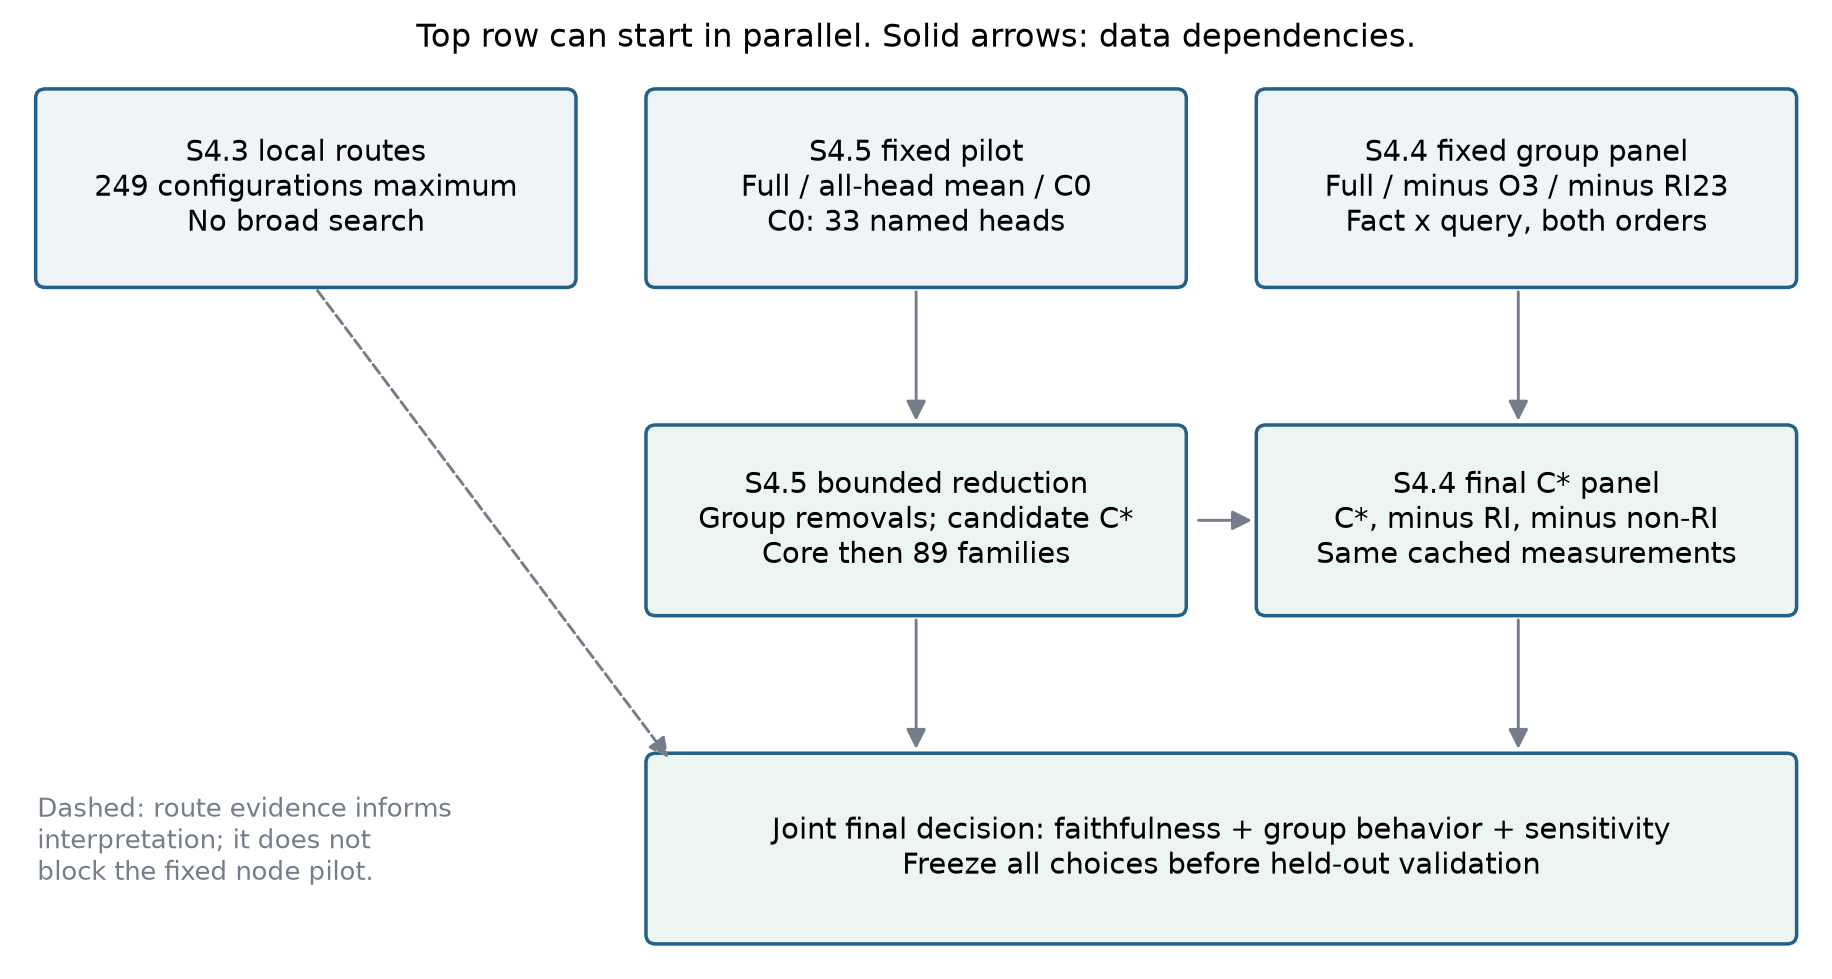
\includegraphics[width=\linewidth]{figures/s42_dependencies.png}
\caption{Proposed execution dependencies. S4.3 local routes, the fixed S4.5 pilot and the three full-model S4.4 configurations can be implemented and run independently. The final C-based semantic configurations necessarily wait for the selected mask. All analyses share the endpoint registry.}
\label{fig:s42_dependencies}
\end{figure}

\begin{enumerate}
\item \textbf{Prepare once:} validate the shared registry, reconstruct the four input cells, reuse original baselines/means and collect missing mean-head statistics. Freeze the named groups, masks, thresholds and compute caps before observing new effects.
\item \textbf{Parallel fixed work:} run the bounded S4.3 panel, the full/all-head-mean/$C_0$ pilot, and the three full-model S4.4 group configurations. No S4.3 outcome is required to begin these fixed node tests. A six-GPU allocation can use three disjoint two-GPU workers; actual family shards and waves should reflect the model memory requirement and dependencies.
\item \textbf{Adaptive S4.5 work:} the pilot determines whether $C_0$ or the single $C_{50}$ fallback qualifies; reduction then determines $C^*$. Completeness/addback and full-discovery checks can change that mask. The framework can be implemented in advance, but the exact endpoint list and retained membership cannot honestly be fixed before these results.
\item \textbf{Dependent S4.4 cells:} fill the three C-based configurations for the selected mask, reusing already measured original-axis cells. Combine their behavioral checks with the S4.5 faithfulness/completeness decision and final donor sensitivity. If C changes during this process, recompute only cells whose complete intervention identity changed.
\item \textbf{Interpret and freeze:} use the local-route results to describe which ordered communications are supported and which remain unresolved. A node mask can be faithful without all its incoming routes being explained, but the report must distinguish these claims. Freeze the chosen mask, group rosters, routes, signs and all validation choices before opening held-out families.
\end{enumerate}

The S4.3 result may change the \emph{interpretation and supported route list}, and may motivate an explicitly recorded finite addback or a later positional refinement. It is not a mandatory computational barrier before the $C_0$ pilot. A new head outside the named pools, automatic whole-block splitting, a second local round, or a broad search is outside this revised plan. If the bounded candidate set fails, that is a legitimate incomplete-mechanism outcome. This prevents an implicit, unbounded dependency from hiding behind the word ``adaptive.''

\textbf{Compute accounting.} The local panel is bounded at 249 scientific configurations (at most 9,960 initial noising endpoints on 40 pairs), plus at most 2,240 matched-direct endpoints before compatible reuse. Gates and selected extensions are additional. The first three S4.4 configurations require at most $3\times40\times4=480$ endpoints on the core crossed panel before reuse; all six require at most 960. The reduction has a separate 96-mask core cap (at most 7,680 two-condition endpoints), and final discovery/paired-baseline/completeness records are scheduled only after the mask is known. Missing-head mean collection, gates and newly tokenized intact baselines are explicit additional work. These are bounded workload counts, not a promised wall-clock duration or a GPU cost quote.

\textbf{What the restructuring saves.} S4.4 owns the behavioral questions and S4.5 owns retention/completeness selection, but neither owns a separate copy of a model forward. Core/full-discovery cells, order variants, group removals and final baseline comparisons are cached once. CPU code derives interactions, paired intervals, accuracy guards and graphs from those records. It cannot infer a new nonlinear group intervention, retained-C background or changed-query endpoint from old singles; such missing configurations still need model computation.
\FloatBarrier

\section{Current conclusion and stopping boundary}
S4.2 moves the project from separately measured routes to tested group dependence. The layer-18 pair is repeatedly important; L17H1's effect depends strongly on the selected receiver group; conditional RI participation is real but heterogeneous; and L26H31 is not supported as the proposed backup. Order and replacement baseline materially affect the conclusions. These findings justify a small set of exact local route tests and a joint group-level behavioral/retention workflow, rather than a new broad search.

The next experiments can test whether a finite head subset preserves the observed computation, which group removals distinguish it from the full model, and whether the same group mechanism follows fact and query changes. They may also return an incomplete or baseline-dependent explanation. No new GPU run, follow-up implementation, full circuit claim or held-out conclusion is included in this report.
